\documentclass{article}
\usepackage[utf8]{inputenc}
\usepackage[hungarian]{babel}

\usepackage{amsmath}

\usepackage{lipsum}
\usepackage{graphicx} % for the includegrapichs
\usepackage{titling}

\usepackage{fancyhdr} % for the header on the first page
\usepackage{pdfpages} % to include pdf
\usepackage{structuralanalysis} % for the figures
\usepackage{tikz-dimline}
\usepackage{wasysym}



\usepackage{multicol}
\usepackage{t1enc}
\usepackage{textcomp}

\newcommand{\rpm}{\raisebox{.2ex}{$\scriptstyle\pm$}}

\begin{document}
	
	\begin{titlepage}
		\setlength{\headheight}{20pt}
		\lhead{
\includegraphics[height=1.5cm]{logo_mm.png}}
		\rhead{\large{\textbf{Végeselem módszer alapjai}}\\
			BMEGEMMAGMV}
		%\vspace{15cm}
		\title{\huge Kötelező házi feladat 2
		}
		\author{Tar Dániel\\GUTOY7}
		\date{\today}
		\maketitle
		\pagenumbering{gobble}
		\thispagestyle{fancy}
		
		\begin{figure}
			\begin{center}
				
\includegraphics[height=2cm]{logo_bme_kicsi.eps}
			\end{center}
		\end{figure}
		
	\end{titlepage}
	\newpage

	%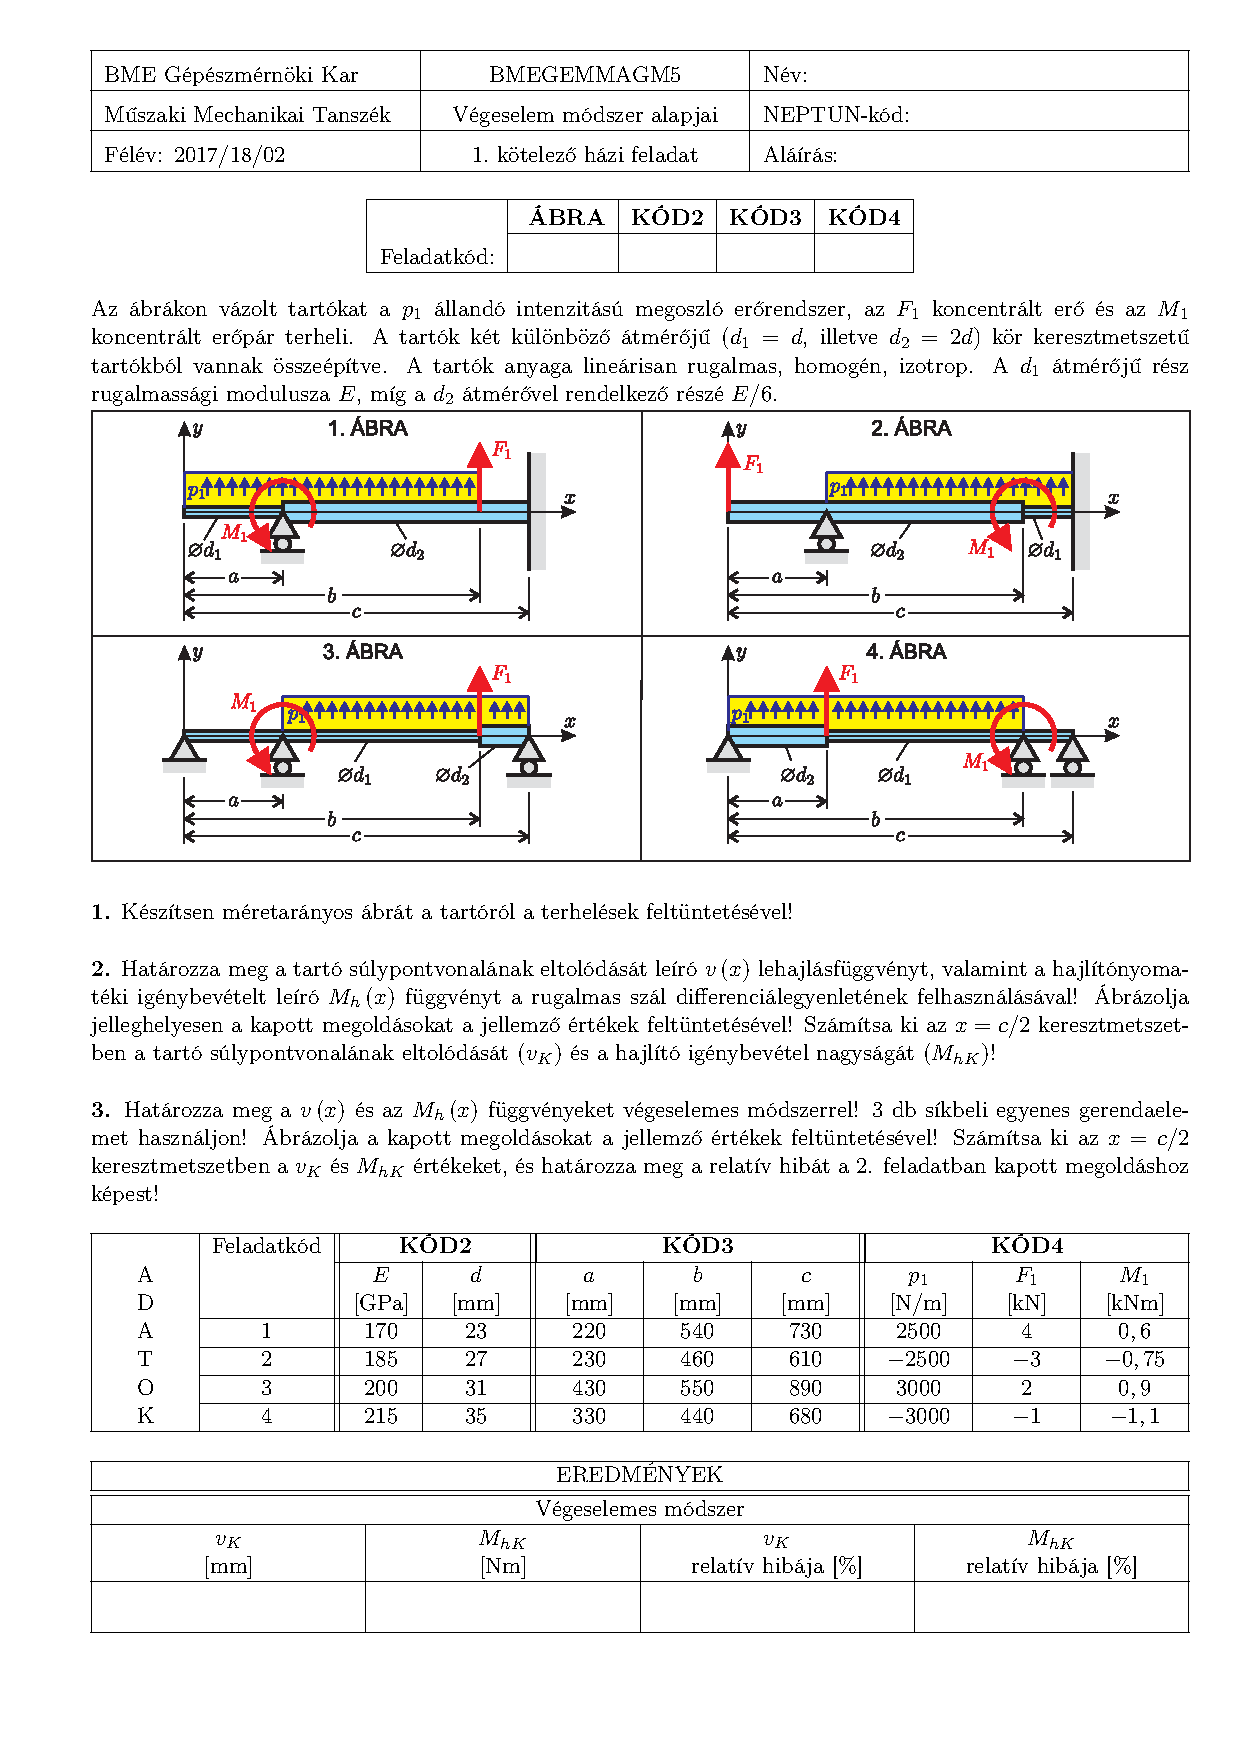
\includepdf{vemalaphf1.pdf}
	 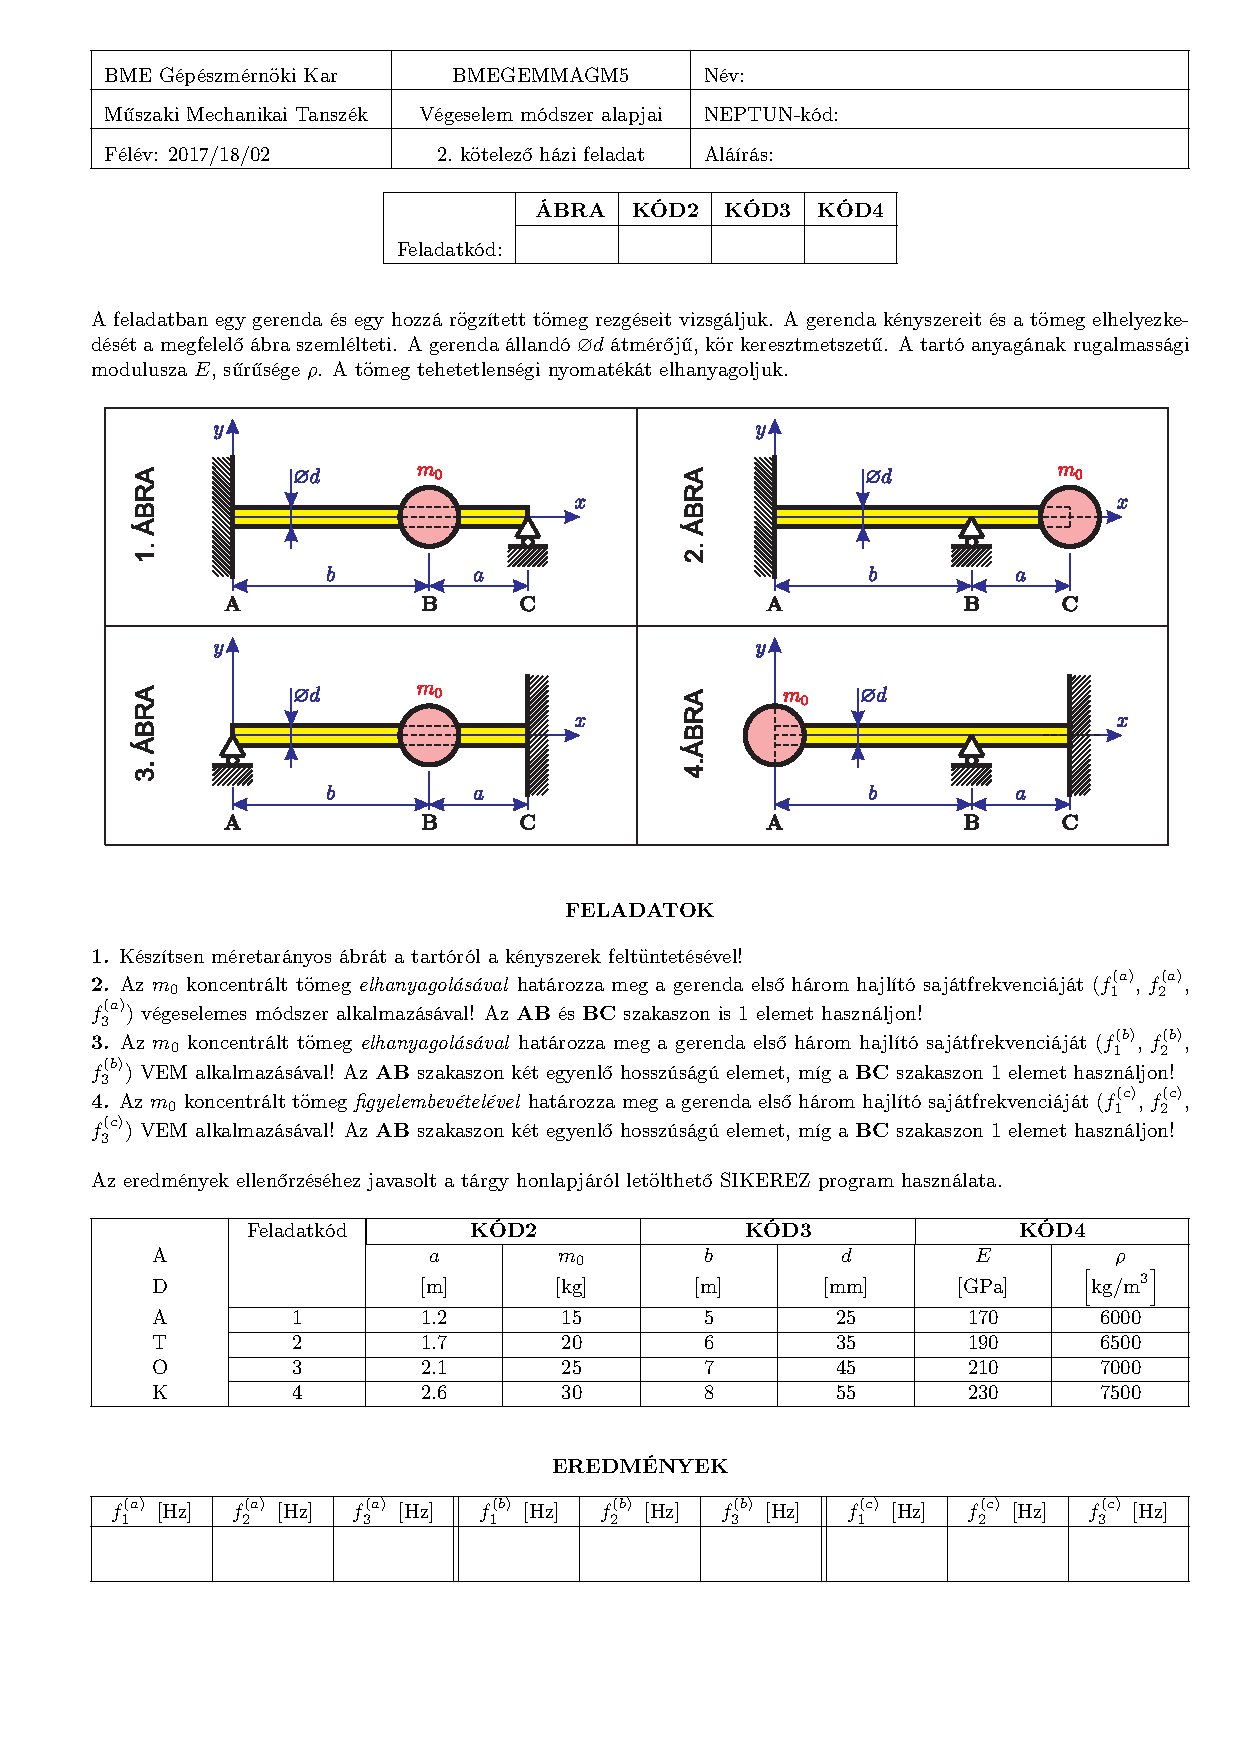
\includepdf[picturecommand*={
	    	\put(460,759){Tar Dániel}
	    	\put(460,742){GUTOY7}
	    	\put(280,680){2}
	    	\put(325,680){1}
	    	\put(368,680){2}
	    	\put(410,680){2}
	 }]{vemalaphf4.pdf}
	\newpage
	
	
	\setlength{\headheight}{0pt}
	\tableofcontents
	\newpage
	
	\pagenumbering{arabic}	
	\setcounter{page}{1}

	
	
	

	
	%\newpage
	
	%---------------------
	% 1.feladat
	%---------------------
	\section{Feladat}
	
	A házifeladat kód alapján az adatok SI mértékegységrendszerben:
	\def\arraystretch{1.2}%
	\begin{table}[h!]
		\begin{center}
			\caption{Adatok}
			\label{tab:table1}
			\begin{tabular}{c|c|c|c|c|c} % <-- Alignments: 1st column left, 2nd middle and 3rd right, with vertical lines in between
				$a$ & $m_{0}$ & $b$ & $d$ & $E$ & $\rho$\\
				$[m]$ & $[kg]$ & $[m]$ & $[m]$ & $[Pa]$ & $[kg/m^{3}]$\\
				\hline
				1,2 & 15 & 6 & 35 & $190\cdot10^3$ & 6500\\
				%2 & 10.1 & b\\
				%3 & 23.113231 & c\\
			\end{tabular}
		\end{center}
	\end{table}
	\def\arraystretch{1}%
	
	Továbbá a rúd keresztmetszetének a felülete:
	\begin{equation}
	A=\frac{d^{2}\cdot\pi}{4}=9,6211 \cdot 10^{-4}~[m^{2}]
	\end{equation}
	
	És a másodrendű nyomatéka:
	\begin{equation}
	I_{z}=\frac{d^4\cdot\pi}{64}=7,3662 \cdot 10^{-8}~[m^{4}]
	\end{equation}
	
	Méretarányos ábra és a kényszerek:
	
	%\newcommand{\newCommandName}{text to insert}
	\newcommand{\sugar}{2}
	\newcommand{\ab}{600}
	\newcommand{\bc}{120}
	\newcommand{\acv}{701}
	\newcommand{\ac}{720}
	\newcommand{\acvv}{735}
	
	
	\begin{figure}[h!]		
		\begin{center}
			\begin{tikzpicture}
				\scaling{.015};
				
				% x and y axis
				\draw[->] (0,0)--(12,0) node[right]{$x$};
				\draw[->] (0,0)--(0,2) node[above]{$y$};
				
				% auxiliary points
				\point{a}{0}{0};
				\point{a1}{0}{-\sugar};
				\point{a2}{0}{\sugar};
				
				\point{b}{\ab}{0};
				\point{c}{\ac}{0};
				\point{c1}{\acv}{-\sugar};
				\point{c2}{\acv}{\sugar};
				\point{d}{200}{0};
				\point{d2}{210}{35};
				
				\draw[thick] (c) circle (0.3cm);
				\draw (d) -- (d2);
				
				% stucture
				\beam{2}{a1}{c1};
				\beam{2}{a2}{c2};
				
				%\support{type}{insertion point}[rotation];
				\support{2}{b};
				\support{3}{a}[-90];
				
				\notation{1}{a}{$A$}[below=8mm];
				\notation{1}{b}{$B$}[below=10mm];
				\notation{1}{c}{$C$}[below=10mm];
				\notation{1}{d2}{$\diameter35~mm$}[above];
				\notation{1}{c2}{$m_{0}$}[above right=2mm];
				
				% dimensions
				\dimensioning{1}{a}{b}{-1.8}[$6~m$];
				\dimensioning{1}{b}{c}{-1.8}[$1.2~m$];
				%\dimensioning{2}{c1}{c2}{-1}[35];
				%\dimensioning{2}{f}{e}{-1}[$54$];		
			\end{tikzpicture}
		\end{center}	
	\caption{}
	\end{figure}
	
	\newpage
	
	%---------------------
	% 2.feladat
	%---------------------
	\section{Feladat}
	
	\subsection{Végeselem modell az $m_{0}$ tömeg elhanyagolásával és az \textbf{AB} szakaszon 1 elem használatával}
	
	\begin{figure}[h!]		
		\begin{center}	
			\begin{tikzpicture}
				\scaling{.015};
				% auxiliary points
				\point{a}{0}{0};
				\point{b}{\ab}{0};
				\point{c}{\acvv}{0};
				\point{d}{200}{0};
				\point{d2}{210}{35};
				
				\beam{2}{a}{b};
				\beam{2}{b}{c};
				
				\support{2}{b};
				\support{3}{a}[-90];
				
				%\hinge{1}{a};
				\hinge{1}{b};
				\hinge{1}{c};
				
				\notation{1}{a}{$(1)$}[above right];
				\notation{1}{b}{$(2)$}[above];
				\notation{1}{c}{$(3)$}[above];
				
				\notation{5}{a}{b}[$I, E, A, \rho $][.5][below];
				\notation{5}{b}{c}[$I, E, A, \rho $][.5][below];
				
				\notation{4}{a}{b}[1]
				\notation{4}{b}{c}[2] 
			\end{tikzpicture}
		\end{center}	
	\caption{}
	\end{figure}
	
	\subsection{A rúdelemek paraméteres elemi mátrixai, és 2x2-es almátrixokkal való helyettesítése}
	
	
		Az elemi merevségi mátrix:
		\begin{equation}
		K_{e,4\times4}= \frac{I_{z} \cdot E}{L^3}  
		\begin{bmatrix}
		12&6L&-12&6L\\
		6L&4L^2&-6L&2L^2\\
		-12&-6L&12&-6L\\
		6L&2L^2&-6L&4L^2\\
		\end{bmatrix}
		=\begin{bmatrix}
		K_{11} &K_{12} \\
		K_{21} &K_{22} \\
		\end{bmatrix}
		\end{equation}
		
		Az elemi tömegmátrix:
		\begin{equation}
		M_{e,4\times4}= \frac{\rho \cdot A \cdot L}{420}  
		\begin{bmatrix}
		156&22L&54&-13L\\
		22L&4L^2&13L&-3L^2\\
		54&13L&156&-22L\\
		-13L&-3L^2&-22L&4L^2\\
		\end{bmatrix}
		=\begin{bmatrix}
		M_{11} &M_{12} \\
		M_{21} &M_{22} \\
		\end{bmatrix}
		\end{equation}
	
	
	
	\subsection{A globális merevségi- és tömegmátrixok összállítása}
		
		Globális merevségi mátrix:
		\begin{equation}
			K_{G,6\times6}=
			\begin{bmatrix}
			K_{11}^{(1)} & K_{12}^{(1)}              & 0            \\
			K_{21}^{(1)} & K_{22}^{(1)}+K_{11}^{(2)} & K_{12}^{(2)} \\
			0            & K_{21}^{(2)}              & K_{22}^{(2)} \\
			\end{bmatrix}
		\end{equation}
		
		Globális tömegmátrix mátrix:
		\begin{equation}
			M_{G,6\times6}=
			\begin{bmatrix}
			M_{11}^{(1)} & M_{12}^{(1)}              & 0            \\
			M_{21}^{(1)} & M_{22}^{(1)}+M_{11}^{(2)} & M_{12}^{(2)} \\
			0            & M_{21}^{(2)}              & M_{22}^{(2)} \\
			\end{bmatrix}
		\end{equation}
	 
	
	\subsection{A mátrixok kondenzálása a lekötött szabadsági fokok alapján}
	
		Lekötött szabadsági fokok:
		
		\[V_{1}=0 \qquad \Phi_{1}=0 \qquad V_{2}=0\]	
	
		Az elmozdulásvektor:
		
		\begin{equation}
			U=
			\begin{bmatrix}
			V_{1}    \\
			\Phi_{1} \\
			V_{2}    \\
			\Phi_{2} \\
			V_{3}    \\
			\Phi_{3} \\
			\end{bmatrix}
			=
			\begin{bmatrix}
			0  \\
			0 \\
			0    \\
			\Phi_{2} \\
			V_{3}    \\
			\Phi_{3} \\
			\end{bmatrix}
		\end{equation}
		
		A kondenzált merevségi mátrix: 
		\begin{equation}
			K_{G,K,3\times3}=
			\begin{bmatrix}
			 K_{G_{44}}	 & K_{G_{45}}	 & K_{G_{46}}   \\
			 K_{G_{54}}	 & K_{G_{55}}	 & K_{G_{56}}   \\
			 K_{G_{64}}	 & K_{G_{65}}	 & K_{G_{66}}   \\
			\end{bmatrix}
		\end{equation}
		
		A kondenzált merevségi mátrix: 
		\begin{equation}
			M_{G,K,3\times3}=
			\begin{bmatrix}
			 M_{G_{44}}	 & M_{G_{45}}	 & M_{G_{46}}   \\
			 M_{G_{54}}	 & M_{G_{55}}	 & M_{G_{56}}   \\
			 M_{G_{64}}	 & M_{G_{65}}	 & M_{G_{66}}   \\
			\end{bmatrix}
		\end{equation}
		
		A kondenzált elmozdulásvektor:
		\begin{equation}
			U_K=
			\begin{bmatrix}
				\Phi_{2} \\
				V_{3}    \\
				\Phi_{3} \\
			\end{bmatrix}
		\end{equation} 
	
	\subsection{A sajátkörfrekvenciák számítása az órán tanult képlet segítségével}
	
		\begin{equation}
			det(K_{G,K} - \omega^2 \cdot M_{G,K}) = 0
		\end{equation}
		
		A sajátértékenként az $\omega^2$-eket kapjuk, majd ebből a sajátfrekvenciák:
		
		\begin{equation}
			f_{1,2,3}=\frac{\omega_{1,2,3}}{2\cdot \pi}
		\end{equation}
		
		Amivel a sajátfrekvenciák:	
		\[f_1^a=3,7712~[Hz] \qquad f_2^a=20,8972~[Hz] \qquad f_3^a=182,5774~[Hz]  \]
		
		Az eredményeim 3 tizedesjegyig teljesen megegyeznek a Sikerez nevű programmal számolt adatokkal, csak az utolsó (4.) tizedesjegyben van \rpm1 eltérés. 
		
				
		A további feladatokat az előző analógiájaként végezhetjük el, az elv ugyan az. 
		Csak a különbségeket és az eredményeket fogom részletezni.
	
	
	%---------------------
	% 3.feladat
	%---------------------
	\section{Feladat}
		
	\subsection{Végeselem modell az $m_{0}$ tömeg elhanyagolásával és az \textbf{AB} szakaszon 2 elem használatával}
	
		\begin{figure}[h!]		
			\begin{center}	
				\begin{tikzpicture}
					\scaling{.015};
					% auxiliary points
					\point{a}{0}{0};
					\point{b}{\ab}{0};
					\point{b1}{\ab/2}{0};
					\point{c}{\acvv}{0};
					\point{d}{200}{0};
					\point{d2}{210}{35};
					
					\beam{2}{a}{b1};
					\beam{2}{b1}{b};
					\beam{2}{b}{c};
					
					\support{2}{b};
					\support{3}{a}[-90];
					
					%\hinge{1}{A};
					\hinge{1}{b1};
					\hinge{1}{b};
					\hinge{1}{c};
					
					\notation{1}{a}{$(1)$}[above right];
					\notation{1}{b1}{$(2)$}[above];
					\notation{1}{b}{$(3)$}[above];
					\notation{1}{c}{$(4)$}[above];
					
					\notation{5}{a}{b1}[$I, E, A, \rho $][.5][below];
					\notation{5}{b1}{b}[$I, E, A, \rho $][.5][below];
					\notation{5}{b}{c}[$I, E, A, \rho $][.5][below];
					
					\notation{4}{a}{b1}[1]
					\notation{4}{b1}{b}[2]
					\notation{4}{b}{c}[3] 
				\end{tikzpicture}
			\end{center}	
		\caption{}
		\end{figure}
	
	
		\subsection{A rúdelemek paraméteres elemi mátrixai, és 2x2-es almátrixokkal való helyettesítése}
	
		Lásd a 2.2-es pontnál.
	
		\subsection{A globális merevségi- és tömegmátrixok összállítása}
		
			Globális merevségi mátrix:
			\begin{equation}
				K_{G,8\times8}=
				\begin{bmatrix}
				K_{11}^{(1)} & K_{12}^{(1)}              & 0            			    & 0            \\
				K_{21}^{(1)} & K_{22}^{(1)}+K_{11}^{(2)} & K_{12}^{(2)}  			    & 0            \\
				0            & K_{21}^{(2)}              & K_{22}^{(2)} + K_{11}^{(3)}  & K_{12}^{(3)} \\
				0            & 0						 & K_{21}^{(3)} 					& K_{22}^{(3)} \\
				\end{bmatrix}
			\end{equation}
			
			Globális tömegmátrix mátrix:
			\begin{equation}
			M_{G,8\times8}=
			\begin{bmatrix}
			M_{11}^{(1)} & M_{12}^{(1)}              & 0            			    & 0            \\
			M_{21}^{(1)} & M_{22}^{(1)}+M_{11}^{(2)} & M_{12}^{(2)}  			    & 0            \\
			0            & M_{21}^{(2)}              & M_{22}^{(2)} + M_{11}^{(3)}  & M_{12}^{(3)} \\
			0            & 0						 & M_{21}^{(3)} 					& M_{22}^{(3)} \\
			\end{bmatrix}
			\end{equation}
	
	
		\subsection{A mátrixok kondenzálása a lekötött szabadsági fokok alapján}
		
			Lekötött szabadsági fokok:
			
			\[V_{1}=0 \qquad \Phi_{1}=0 \qquad V_{3}=0\]	
			
			Az elmozdulásvektor:
			
			\begin{equation}
				U=
				\begin{bmatrix}
				V_{1}    \\
				\Phi_{1} \\
				V_{2}    \\
				\Phi_{2} \\
				V_{3}    \\
				\Phi_{3} \\
				V_{4}    \\
				\Phi_{4} \\
				\end{bmatrix}
				=
				\begin{bmatrix}
				0  \\
				0 \\
				V_{2}    \\
				\Phi_{2} \\
				0   \\
				\Phi_{3} \\
				V_{4}    \\
				\Phi_{4} \\
				\end{bmatrix}
			\end{equation}
			
			A kondenzált merevségi mátrix: 
			\begin{equation}
				K_{G,K,5\times5}=
				\begin{bmatrix}
				K_{G_{33}}	 & K_{G_{34}}	 & K_{G_{36}} & K_{G_{37}}	 & K_{G_{38}}  \\
				K_{G_{43}}	 & K_{G_{44}}	 & K_{G_{46}} & K_{G_{47}}	 & K_{G_{48}}  \\
				K_{G_{63}}	 & K_{G_{64}}	 & K_{G_{66}} & K_{G_{67}}	 & K_{G_{68}}  \\
				K_{G_{73}}	 & K_{G_{74}}	 & K_{G_{76}} & K_{G_{77}}	 & K_{G_{78}}  \\
				K_{G_{83}}	 & K_{G_{84}}	 & K_{G_{86}} & K_{G_{87}}	 & K_{G_{88}}  \\
				\end{bmatrix}
			\end{equation}
			
			A kondenzált merevségi mátrix: 
			\begin{equation}
				M_{G,M,5\times5}=
				\begin{bmatrix}
				M_{G_{33}}	 & M_{G_{34}}	 & M_{G_{36}} & M_{G_{37}}	 & M_{G_{38}}  \\
				M_{G_{43}}	 & M_{G_{44}}	 & M_{G_{46}} & M_{G_{47}}	 & M_{G_{48}}  \\
				M_{G_{63}}	 & M_{G_{64}}	 & M_{G_{66}} & M_{G_{67}}	 & M_{G_{68}}  \\
				M_{G_{73}}	 & M_{G_{74}}	 & M_{G_{76}} & M_{G_{77}}	 & M_{G_{78}}  \\
				M_{G_{83}}	 & M_{G_{84}}	 & M_{G_{86}} & M_{G_{87}}	 & M_{G_{88}}  \\
				\end{bmatrix}
			\end{equation}
			
			A kondenzált elmozdulásvektor:
			\begin{equation}
				U_K=
				\begin{bmatrix}
				V_{2}    \\
				\Phi_{2} \\
				\Phi_{3} \\
				V_{4}    \\
				\Phi_{4} \\
				\end{bmatrix}
			\end{equation} 
	
	\subsection{A sajátkörfrekvenciák számítása az órán tanult képlet segítségével}
	
		\begin{equation}
			det(K_{G,K} - \omega^2 \cdot M_{G,K}) = 0
		\end{equation}
		
		A sajátértékenként az $\omega^2$-eket kapjuk, majd ebből a sajátfrekvenciák:
		
		\begin{equation}
			f_{1,2,3}=\frac{\omega_{1,2,3}}{2\cdot \pi}
		\end{equation}
		
		Amivel a sajátfrekvenciák:	
		\[f_1^b=3,1038~[Hz] \qquad f_2^b=8,8729~[Hz] \qquad f_3^b=17,4725~[Hz]  \]
		
		Az eredményeim 3 tizedesjegyig teljesen megegyeznek a Sikerez nevű programmal számolt adatokkal, csak az utolsó (4.) tizedesjegyben van \rpm1 eltérés. 
	
	%---------------------
	% 4.feladat
	%---------------------
	\section{Feladat}
	
		\subsection{Végeselem modell az \textbf{AB} szakaszon 2 elem használatával:}
	
			\begin{figure}[h!]		
				\begin{center}
					\begin{tikzpicture}
					\scaling{.015};
					% auxiliary points
					\point{a}{0}{0};
					\point{b}{\ab}{0};
					\point{b1}{\ab/2}{0};
					\point{c}{\acvv}{0};
					\point{d}{200}{0};
					\point{d2}{210}{35};
					
					\beam{2}{a}{b1};
					\beam{2}{b1}{b};
					\beam{2}{b}{c};
					
					\support{2}{b};
					\support{3}{a}[-90];
					
					%\hinge{1}{A};
					\hinge{1}{b1};
					\hinge{1}{b};
					\hinge{1}{c};
					
					\notation{1}{a}{$(1)$}[above right];
					\notation{1}{b1}{$(2)$}[above];
					\notation{1}{b}{$(3)$}[above];
					\notation{1}{c}{$(4)$}[above=0.25];
					\notation{1}{c}{$m_0$}[right=0.4];
					
					\notation{5}{a}{b1}[$I, E, A, \rho $][.5][below];
					\notation{5}{b1}{b}[$I, E, A, \rho $][.5][below];
					\notation{5}{b}{c}[$I, E, A, \rho $][.5][below];
					
					\notation{4}{a}{b1}[1]
					\notation{4}{b1}{b}[2]
					\notation{4}{b}{c}[3] 
					
					\draw[thick, inner color=white] (c) circle (3.5mm);
					
					\end{tikzpicture}
				\end{center}	
			\caption{}
			\end{figure}
	
		\subsection{A rúdelemek paraméteres elemi mátrixai, és 2x2-es almátrixokkal való helyettesítése}
		
			Lásd a 2.2-es pontnál.
		
		\subsection{A globális merevségi- és tömegmátrixok összállítása}
		
			Globális merevségi mátrix:
			\begin{equation}
				K_{G,8\times8}=
				\begin{bmatrix}
					K_{11}^{(1)} & K_{12}^{(1)}              & 0            			    & 0            \\
					K_{21}^{(1)} & K_{22}^{(1)}+K_{11}^{(2)} & K_{12}^{(2)}  			    & 0            \\
					0            & K_{21}^{(2)}              & K_{22}^{(2)} + K_{11}^{(3)}  & K_{12}^{(3)} \\
					0            & 0						 & K_{21}^{(3)} 				& K_{22}^{(3)} \\
				\end{bmatrix}
			\end{equation}
		
			Globális tömegmátrix mátrix:
			\begin{equation}
				M_{G,8\times8}=
					\begin{bmatrix}
					M_{11}^{(1)} & M_{12}^{(1)}              & 0            			    & 0            \\
					M_{21}^{(1)} & M_{22}^{(1)}+M_{11}^{(2)} & M_{12}^{(2)}  			    & 0            \\
					0            & M_{21}^{(2)}              & M_{22}^{(2)} + M_{11}^{(3)}  & M_{12}^{(3)} \\
					0            & 0						 & M_{21}^{(3)} 				& M_{22}^{(3)} \\
					\end{bmatrix}
			\end{equation}
			
			A globális merevségi mátrixhoz hozzá kell adnunk a tömeget is, úgy, hogy elhanyagoljuk a nyomatékát. A tömeg a (4)-es pontban található, ezért a globális tömegmátrix [7,7] eleméhez adjuk hozzá:
			
			\begin{equation}
				M_G[7,7] = M_G[7,7] + m_0
			\end{equation}
		
		
		\subsection{A mátrixok kondenzálása a lekötött szabadsági fokok alapján}
		
			Lekötött szabadsági fokok, és a kondenzálás folyamata ugyon az mint a 3.4-es feladatnál.
		
		\subsection{A sajátkörfrekvenciák számítása az órán tanult képlet segítségével}
	
			\begin{equation}
				det(K_{G,K} - \omega^2 \cdot M_{G,K}) = 0
			\end{equation}
			
			A sajátértékenként az $\omega^2$-eket kapjuk, majd ebből a sajátfrekvenciák:
			
			\begin{equation}
				f_{1,2,3}=\frac{\omega_{1,2,3}}{2\cdot \pi}
			\end{equation}
			
			Amivel a sajátfrekvenciák:	
			\[f_1^c=2,2813~[Hz] \qquad f_2^c=5,0735~[Hz] \qquad f_c^b=15,1727~[Hz]  \]
			
			Az eredményeim 3 tizedesjegyig teljesen megegyeznek a Sikerez nevű programmal számolt adatokkal, csak az utolsó (4.) tizedesjegyben van \rpm1 eltérés.

\end{document}
